\begin{frame}[allowframebreaks]{ConvNeXt: A Modern CNN}
    \begin{itemize}
        \item ConvNeXt is a modern CNN architecture that incorporates insights from transformer models.
        \item It uses a hierarchical design similar to Swin Transformer, with a focus on simplicity and efficiency.
        \item Key features include:
            \begin{itemize}
                \item Depthwise separable convolutions
                \item Layer normalization
                \item Global average pooling
            \end{itemize}
        \item Achieves competitive performance on image classification tasks while maintaining the strengths of CNNs.
        \item ConvNeXt demonstrates that CNNs can still be effective with modern design principles, even in the era of transformers.
    \end{itemize}
    \framebreak
    \begin{figure}
        \centering
        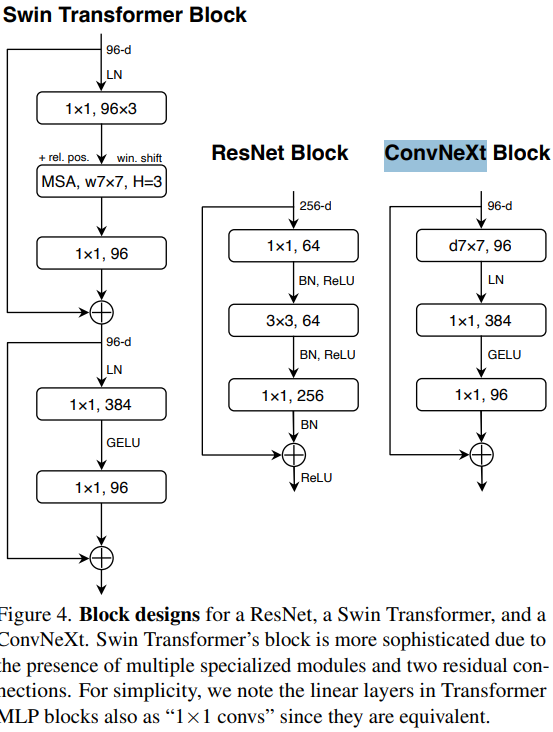
\includegraphics[width=\linewidth,height=0.9\textheight,keepaspectratio]{images/vit/ConvNeXt.png}
        \footnote{Liu et al., “A ConvNet for the 2020s”, CVPR 2022 \url{https://arxiv.org/abs/2201.03545}}
    \end{figure}
\end{frame}